\subsection{Filtrowanie wykresu \PP{}}

Przedmiotem badań w analizie zmienności rytmu serca w oparciu o szeregi odcinków $RR$ jest
rytm zatokowy, nie analizuje się pobudzeń ektopowych czy też artefaktów technicznych.
Rytm serca może być jednak zakłócony przez takie pobudzenia, dlatego zostały
wprowadzone mechanizmy zwane filtrami w celu eliminacji takich niepożądanych informacji. 

Bardzo często te 'nieprawidłowe' pobudzenia są oznaczane przez urządzenia pomiarowe.
Jeśli jednak urządzenia nie posiadają takiej funkcjonalności wtedy stosuje się
specjalistyczne oprogramowanie o dość skomplikowanych algorytmach i niestety nie jest to
rozwiązanie do końca wiarygodne \cite{task2}. Danymi wejściowymi dla takiego oprogramowania
jest pełny zapis EKG, a nie szeregi $RR$.

Mając do dyspozycji szeregi $RR$, z anotacjami sprzętowymi, bardzo ważne jest
wybranie właściwego sposobu filtrowania danych na porzeby wykresów \PP{}.
Poniżej na rysunku \ref{fig:filtr_start} został przedstawiony wektor $RR$ z oznaczonymi
wartościami pochodzącymi od innych źródeł niż węzeł zatokowy.
\begin{figure}
\centering
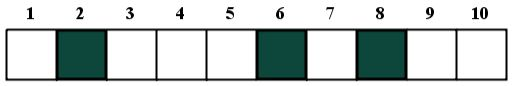
\includegraphics[scale=0.65]{graph/filtr_start.jpg}
\caption{Rysunek przedstawia wektor $RR$ z oznaczonymi, zielone kwadraty, pobudzeniami ektopowymi lub artefaktami technicznymi.}
\label{fig:filtr_start}
\end{figure}

Rysunek \ref{fig:filtr_ewolucja} przedstawia w jaki sposób powinno być przeprowadzone 
filtrowanie danych z anotacjami tak aby uzyskać poprawnie skonstruowane wektory $\bRRm$,
$\bRRn$ dla wykresu \PP{}. Oznaczenia wspólne dla wszystkich paneli: kwadraty czerwone
reprezentują elementy szeregów $RR$ które są usuwane tak aby uzyskać wektory zgodne w
definicją (\ref{eq:wektory2}); kwadraty zielone reprezentują pobudzenia ektopowe
lub artefakty techniczne; wektor po lewej i prawej stronie każdego panelu reprezentuje
ten sam szereg $RR$.

Panel A zawiera dwa wektory bez żadnego filtrowania. Panel B przestawia bardzo proste
filtrowanie polegające na odrzuceniu wszystkich wartości nie mających swojego źródła w
węźle zatokowym, jednakże użycie takiego filtru powoduje że otrzymujemy niepoprawne,
rozpatrując z formalnego punktu widzenia, punkty dla wykresu \PP{}, tzn.:
$(1,3)$, $(5,7)$, $(7,9)$, ponieważ są nieprzylegle i powstają w wyniku zastosowania
takiej a nie innej procedury filtrowania. Panel C, reprezentuje
prawidłowe filtrowanie w którym wektory $\bRRm$, $\bRRn$ są względem siebie przesunięte
o jeden element i wszystkie pary dla których chociaż jeden element ma anotacje zostają
usunięte, wynikiem takiej procedury są pary współrzędnych:
$(3,4)$, $(4,5)$, $(9,10)$, wszystkie zgodne z definicją wykresu \PP{}. Oczywiście
procedura użyta przy konstrukcji panelu C powoduje usunięcie także pewnych wartości
odnoszących się pobudzeń z węzła zatokowego, tym niemniej nie generuje nieprawidłowych
danych dla wykresu \PP{}.

\begin{figure}
\centering
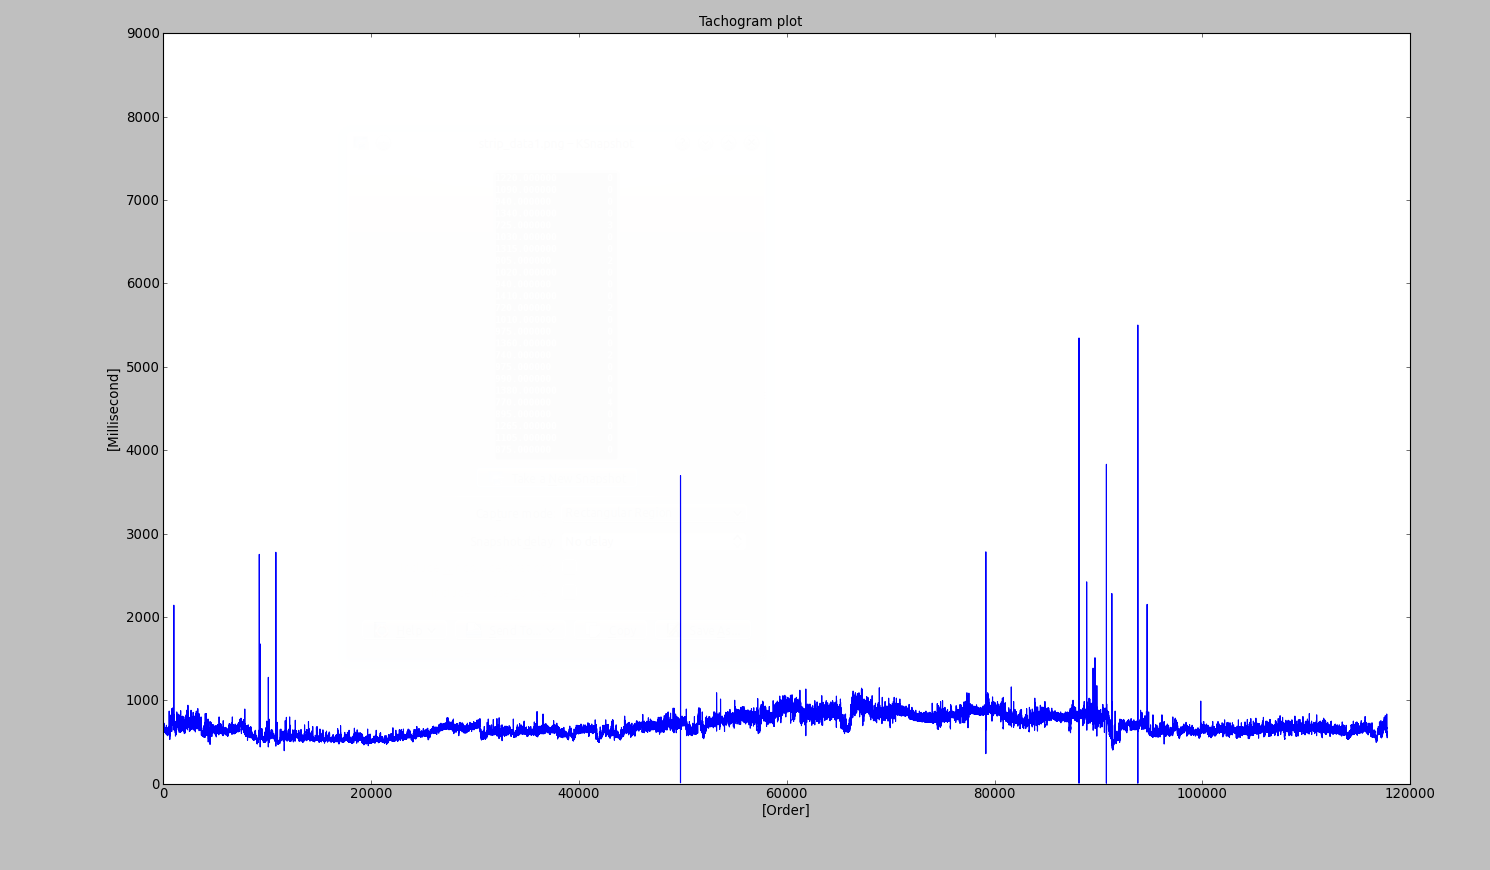
\includegraphics[scale=0.3]{graph/24h_tachogram_unfiltered.png}
\caption{Przykład, tachogram 24 godzinny zapis bez użycia filtra}.
\label{fig:24h_tachogram_unfiltered}
\end{figure}

\begin{figure}
\centering
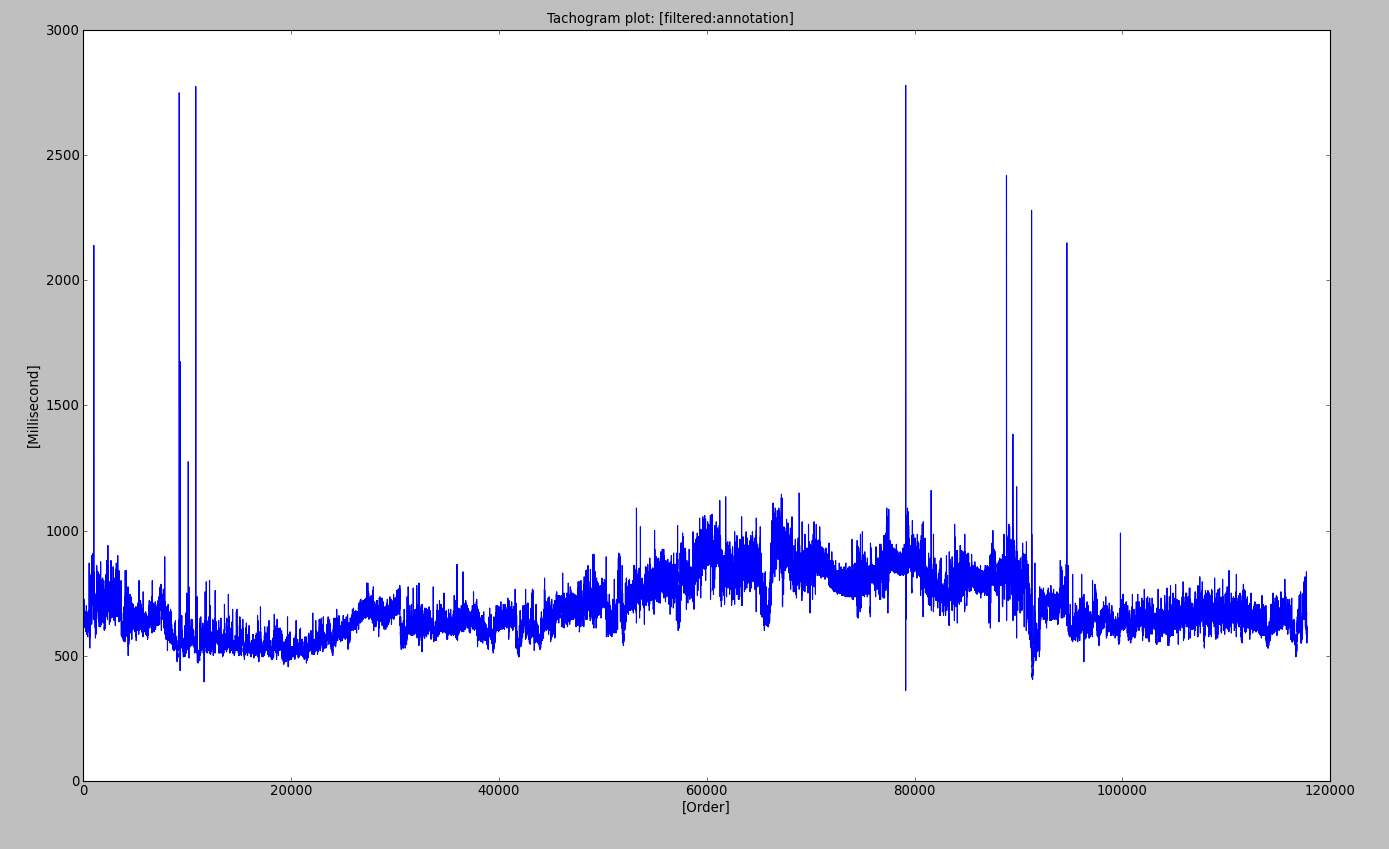
\includegraphics[scale=0.3]{graph/24h_tachogram_annotated.png}
\caption{Przykład, tachogram 24 godzinny zapis z użyciem filtra anotacyjnego}.
\label{fig:24h_tachogram_annotated}
\end{figure}


\begin{figure}
\centering
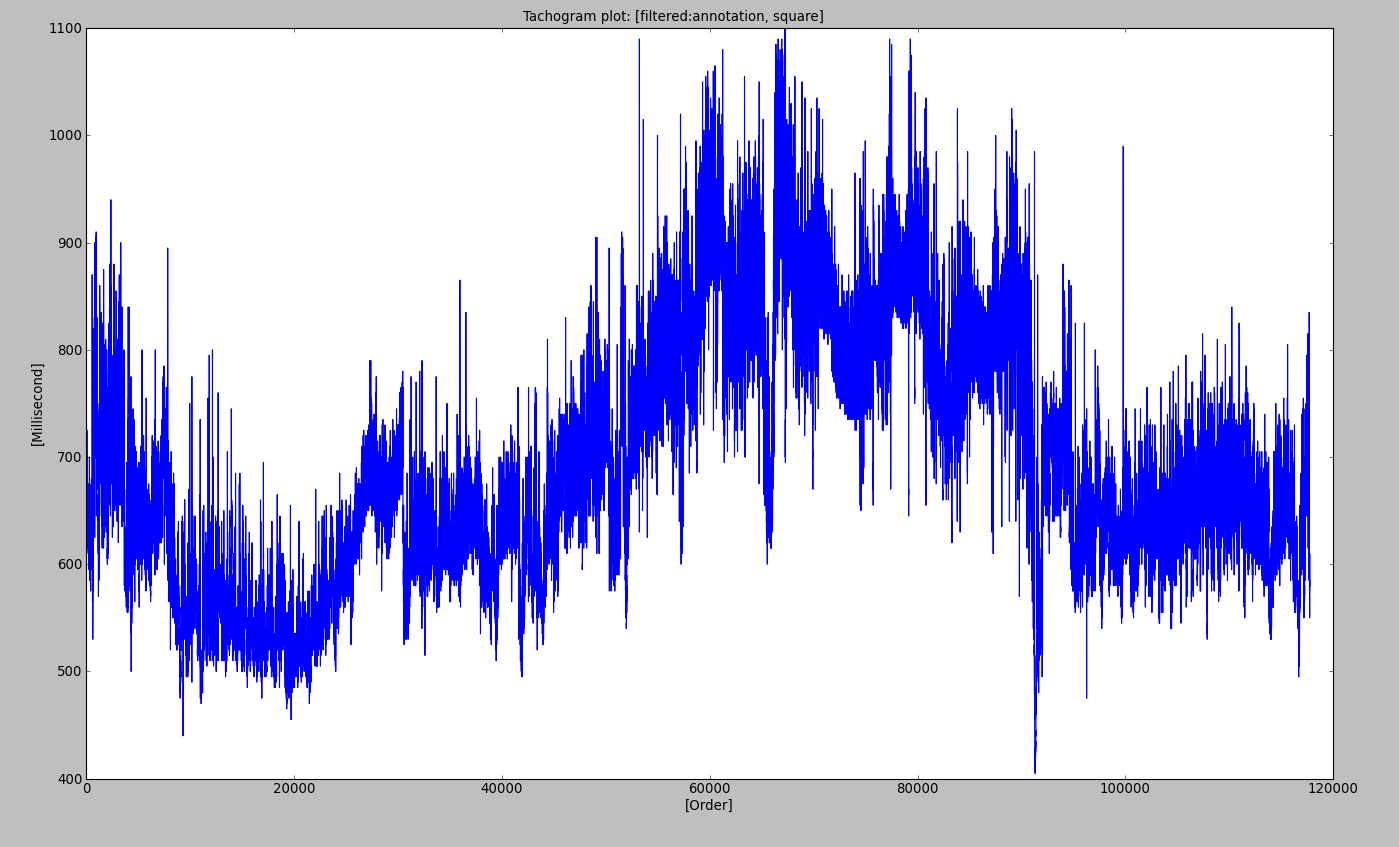
\includegraphics[scale=0.3]{graph/24h_tachogram_annotated_squared.png}
\caption{Przykład, tachogram 24 godzinny zapis z użyciem filtra kwadratowego}.
\label{fig:24h_tachogram_annotated_squared}
\end{figure}

\begin{figure}
\centering
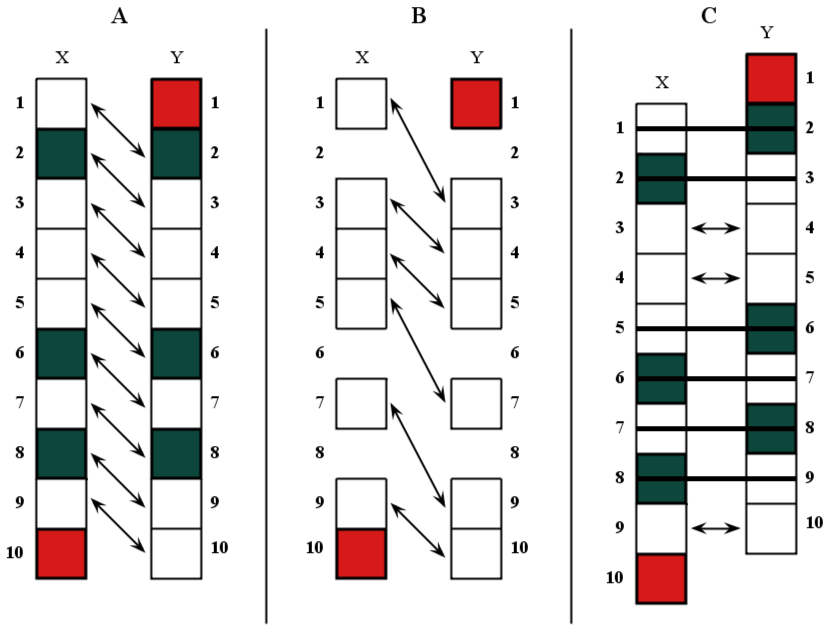
\includegraphics[scale=0.5]{graph/filtr_ewolucja.png}
\caption{Filtrowanie danych dla wykresu \PP{}. Oznaczenie $X$ reprezentuje wektor $\bRRn$,
$Y$ reprezentuje wektor $\bRRp$. Czerwone kwadraty reprezentują usunięte elementy z oryginalnego wektora $RR$ w celu uzyskania odpowiedniego wektora dla wykresu \PP{}.
Zielone kwadraty reprezentują pobudzenia pochodzące z poza węzła zatokowego lub artefakty techniczne. Panel A przestawia wektory $\bRRn$, $\bRRp$ bez filtrowania, panel B z nieprawidłowym filtrowaniem, panel C z prawidłowym filtrowaniem. Szczegóły w tekście.}.
\label{fig:filtr_ewolucja}
\end{figure}

Oto dwa przykłady filtrów:
\subsubsection{Filtr anotacyjny}
Filtr anotacyjny jest przeznaczony do filtrowania wartości szeregu $RR$ z anotacjami.
Przykład takich danych został zaprezentowany na rysunku \ref{fig:strip_data}, gdzie w
drugiej kolumnie sa flagi, anotacje, o następujących wartościach: $0$ - zwykłe uderzenie
z węzła zatokowego, $1$ - uderzenie komorowe, $2$ - uderzenie nadkomorowe, $4$ - artefakt.
Działanie tego filtru jest dokładnie takie samo jak algorytm w wyniku którego uzyskuje się
wektory $\bRRn$, $\bRRp$ w panelu C na rysunku \ref{fig:filtr_ewolucja}.
\begin{verbatim}
UZUPELNIC CODE INFO
pymath.time_domain.poincare_plot.filters.annotation_filter.AnnotationFilter
\end{verbatim}

\subsubsection{Filtr kwadratowy}
Wprowadzenie filtru kwadratowego jest związane z fizjologią rytmu serca. Przyjmuje się
przy analizie elektrokardiogramu, że wszelkie nieprawidłowe dlugości odcinków $RR$
związane z pobudzeniami komorowymi, nadkomorowymi lub wynikające z działania np
rozrusznika serca są zwykle krótsze niż $300$ ms lub dłuższe niż $2000$ ms, zatem jeśli
bierzemy tylko pod uwagę wartości dla pobudzeń zatokowych, warunek odfiltrujący
nieprawidłowe dane możemy symbolicznie zapisać jako:
$\bRRn>300 \wedge \bRRp>300 \wedge \bRRn<2000 \wedge \bRRp<2000$.
Filtr kwadratowy najcześciej stosuje się po użyciu filtra anotacyjnego, ale nie jest to
warunek konieczny.

\begin{verbatim}
UZUPELNIC CODE INFO
pymath.time_domain.poincare_plot.filters.square_filter.SquareFilter
\end{verbatim} 

\begin{figure}
\centering
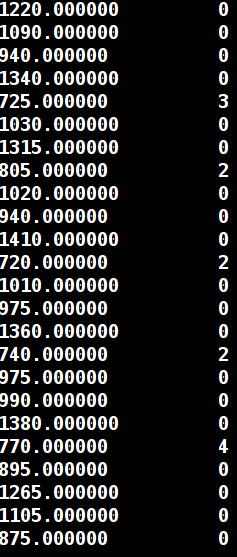
\includegraphics[scale=0.5]{graph/strip_data.png}
\caption{Wycinek danych: pierwsza kolumna wartości $RR$, druga anotacje}.
\label{fig:strip_data}
\end{figure}